%%**************************************************************
%% Vorlage fuer Bachelorarbeiten (o.ä.) der DHBW
%%
%% Autor: Tobias Dreher, Yves Fischer
%% Datum: 06.07.2011
%%
%% Autor: Michael Gruben
%% Datum: 15.05.2013
%%
%% Autor: Markus Barthel
%% Datum: 22.08.2014
%%**************************************************************

%!TEX root = ../dokumentation.tex

%
% Nahezu alle Einstellungen koennen hier getaetigt werden
%

\RequirePackage[l2tabu, orthodox]{nag}	% weist in Commandozeile bzw. log auf veraltete LaTeX Syntax hin

\documentclass[%
	pdftex,
	oneside,			% Einseitiger Druck.
	12pt,				% Schriftgroesse
	parskip=half,		% Halbe Zeile Abstand zwischen Absätzen.
%	topmargin = 10pt,	% Abstand Seitenrand (Std:1in) zu Kopfzeile [laut log: unused]
	headheight = 12pt,	% Höhe der Kopfzeile
%	headsep = 30pt,	% Abstand zwischen Kopfzeile und Text Body  [laut log: unused]
	headsepline,		% Linie nach Kopfzeile.
	footsepline,		% Linie vor Fusszeile.
	footheight = 16pt,	% Höhe der Fusszeile
	abstracton,		% Abstract Überschriften
	DIV=calc,		% Satzspiegel berechnen
	BCOR=8mm,		% Bindekorrektur links: 8mm
	headinclude=false,	% Kopfzeile nicht in den Satzspiegel einbeziehen
	footinclude=false,	% Fußzeile nicht in den Satzspiegel einbeziehen
	listof=totoc,		% Abbildungs-/ Tabellenverzeichnis im Inhaltsverzeichnis darstellen
	toc=bibliography,	% Literaturverzeichnis im Inhaltsverzeichnis darstellen
]{scrreprt}	% Koma-Script report-Klasse, fuer laengere Bachelorarbeiten alternativ auch: scrbook

% Einstellungen laden
\usepackage{xstring}
\usepackage[utf8]{inputenc}
\usepackage[T1]{fontenc}

\newcommand{\einstellung}[1]{%
  \expandafter\newcommand\csname #1\endcsname{}
  \expandafter\newcommand\csname setze#1\endcsname[1]{\expandafter\renewcommand\csname#1\endcsname{##1}}
}
\newcommand{\langstr}[1]{\einstellung{lang#1}}

\einstellung{martrikelnr}
\einstellung{titel}
\einstellung{kurs}
\einstellung{datumAbgabe}
\einstellung{firma}
\einstellung{firmenort}
\einstellung{abgabeort}
\einstellung{abschluss}
\einstellung{studiengang}
\einstellung{dhbw}
\einstellung{betreuer}
\einstellung{gutachter}
\einstellung{zeitraum}
\einstellung{arbeit}
\einstellung{autor}
\einstellung{sprache}
\einstellung{schriftart}
\einstellung{seitenrand}
\einstellung{kapitelabstand}
\einstellung{spaltenabstand}
\einstellung{zeilenabstand}
\einstellung{zitierstil}
 % verfügbare Einstellungen
%%%%%%%%%%%%%%%%%%%%%%%%%%%%%%%%%%%%%%%%%%%%%%%%%%%%%%%%%%%%%%%%%%%%%%%%%%%%%%%
%                                   Einstellungen
%
% Hier können alle relevanten Einstellungen für diese Arbeit gesetzt werden.
% Dazu gehören Angaben u.a. über den Autor sowie Formatierungen.
%
%
%%%%%%%%%%%%%%%%%%%%%%%%%%%%%%%%%%%%%%%%%%%%%%%%%%%%%%%%%%%%%%%%%%%%%%%%%%%%%%%


%%%%%%%%%%%%%%%%%%%%%%%%%%%%%%%%%%%% Sprache %%%%%%%%%%%%%%%%%%%%%%%%%%%%%%%%%%%
%% Aktuell sind Deutsch und Englisch unterstützt.
%% Es werden nicht nur alle vom Dokument erzeugten Texte in
%% der entsprechenden Sprache angezeigt, sondern auch weitere
%% Aspekte angepasst, wie z.B. die Anführungszeichen und
%% Datumsformate.
\setzesprache{de} % oder en
%%%%%%%%%%%%%%%%%%%%%%%%%%%%%%%%%%%%%%%%%%%%%%%%%%%%%%%%%%%%%%%%%%%%%%%%%%%%%%%%

%%%%%%%%%%%%%%%%%%%%%%%%%%%%%%%%%%% Angaben  %%%%%%%%%%%%%%%%%%%%%%%%%%%%%%%%%%%
%% Die meisten der folgenden Daten werden auf dem
%% Deckblatt angezeigt, einige auch im weiteren Verlauf
%% des Dokuments.
\setzemartrikelnr{1577610}
\setzekurs{STG-TINF15-ITA}
\setzetitel{Entwicklung einer App zur Steuerung und Datenauswertung einer Drohne zur Luftqualitätsmessung}
%\setzetitel{Logfileanalyse mit Apache{\textsuperscript{TM}} Hadoop\textsuperscript{{\textregistered}} MapReduce}
\setzedatumAbgabe{04.06.2018}
\setzefirma{Robert Bosch GmbH}
\setzefirmenort{Stuttgart}
\setzeabgabeort{Stuttgart}
\setzeabschluss{nothing}
\setzestudiengang{Informatik}
\setzedhbw{Stuttgart}
\setzebetreuer{Thilo Ackermann, Rene Lasse}
\setzegutachter{nothing}
\setzezeitraum{xx Wochen}
\setzearbeit{Studienarbeit}
\setzeautor{Julian Riegger}
%%%%%%%%%%%%%%%%%%%%%%%%%%%%%%%%%%%%%%%%%%%%%%%%%%%%%%%%%%%%%%%%%%%%%%%%%%%%%%%%

%%%%%%%%%%%%%%%%%%%%%%%%%%%% Literaturverzeichnis %%%%%%%%%%%%%%%%%%%%%%%%%%%%%%
%% Bei Fehlern während der Verarbeitung bitte in ads/header.tex bei der
%% Einbindung des Pakets biblatex (ungefähr ab Zeile 110,
%% einmal für jede Sprache), biber in bibtex ändern.
\newcommand{\ladeliteratur}{%
\addbibresource{bibliographie.bib}
%\addbibresource{weitereDatei.bib}
}
%% Zitierstil
%% siehe: http://ctan.mirrorcatalogs.com/macros/latex/contrib/biblatex/doc/biblatex.pdf (3.3.1 Citation Styles)
%% mögliche Werte z.B numeric-comp, alphabetic, authoryear
\setzezitierstil{authoryear}
%%%%%%%%%%%%%%%%%%%%%%%%%%%%%%%%%%%%%%%%%%%%%%%%%%%%%%%%%%%%%%%%%%%%%%%%%%%%%%%%

%%%%%%%%%%%%%%%%%%%%%%%%%%%%%%%%% Layout %%%%%%%%%%%%%%%%%%%%%%%%%%%%%%%%%%%%%%%
%% Verschiedene Schriftarten
% laut nag Warnung: palatino obsolete, use mathpazo, helvet (option scaled=.95), courier instead
\setzeschriftart{lmodern} % palatino oder goudysans, lmodern, libertine

%% Paket um Textteile drehen zu können
%\usepackage{rotating}
%% Paket um Seite im Querformat anzuzeigen
%\usepackage{lscape}

%% Seitenränder
\setzeseitenrand{2.5cm}

%% Abstand vor Kapitelüberschriften zum oberen Seitenrand
\setzekapitelabstand{20pt}

%% Spaltenabstand
\setzespaltenabstand{10pt}
%%Zeilenabstand innerhalb einer Tabelle
\setzezeilenabstand{1.5}
%%%%%%%%%%%%%%%%%%%%%%%%%%%%%%%%%%%%%%%%%%%%%%%%%%%%%%%%%%%%%%%%%%%%%%%%%%%%%%%%

%%%%%%%%%%%%%%%%%%%%%%%%%%%%% Verschiedenes  %%%%%%%%%%%%%%%%%%%%%%%%%%%%%%%%%%%
%% Farben (Angabe in HTML-Notation mit großen Buchstaben)
\newcommand{\ladefarben}{%
	\definecolor{LinkColor}{HTML}{00007A}
	\definecolor{ListingBackground}{HTML}{FCFAFB}
}
%% Mathematikpakete benutzen (Pakete aktivieren)
\usepackage{amsmath}
\usepackage{amssymb}

%% Programmiersprachen Highlighting (Listings)
\newcommand{\listingsettings}{%
	\lstset{%
		language=Java,			% Standardsprache des Quellcodes
		numbers=left,			% Zeilennummern links
		stepnumber=1,			% Jede Zeile nummerieren.
		numbersep=5pt,			% 5pt Abstand zum Quellcode
		numberstyle=\tiny,		% Zeichengrösse 'tiny' für die Nummern.
		breaklines=true,		% Zeilen umbrechen wenn notwendig.
		breakautoindent=true,	% Nach dem Zeilenumbruch Zeile einrücken.
		postbreak=\space,		% Bei Leerzeichen umbrechen.
		tabsize=2,				% Tabulatorgrösse 2
		basicstyle=\ttfamily\footnotesize, % Nichtproportionale Schrift, klein für den Quellcode
		showspaces=false,		% Leerzeichen nicht anzeigen.
		showstringspaces=false,	% Leerzeichen auch in Strings ('') nicht anzeigen.
		extendedchars=true,		% Alle Zeichen vom Latin1 Zeichensatz anzeigen.
		captionpos=b,			% sets the caption-position to bottom
		backgroundcolor=\color{ListingBackground}, % Hintergrundfarbe des Quellcodes setzen.
		xleftmargin=0pt,		% Rand links
		xrightmargin=0pt,		% Rand rechts
		frame=single,			% Rahmen an
		frameround=ffff,
		rulecolor=\color{darkgray},	% Rahmenfarbe
		fillcolor=\color{ListingBackground},
		keywordstyle=\color[rgb]{0.133,0.133,0.6}\bfseries,
		commentstyle=\color{Sepia},
		stringstyle=\color{red}
	}
}
%%%%%%%%%%%%%%%%%%%%%%%%%%%%%%%%%%%%%%%%%%%%%%%%%%%%%%%%%%%%%%%%%%%%%%%%%%%%%%%%

%%%%%%%%%%%%%%%%%%%%%%%%%%%%%%%% Eigenes %%%%%%%%%%%%%%%%%%%%%%%%%%%%%%%%%%%%%%%
%% Hier können Ergänzungen zur Präambel vorgenommen werden (eigene Pakete, Einstellungen)

% xcolor muss mit optionen vor pdfpages geladen werden
\usepackage[usenames,dvipsnames,table,xcdraw]{xcolor} 	%xcolor für HTML-Notation

\usepackage{pdfpages}
 % lese Einstellungen

\newcommand{\iflang}[2]{%
  \IfStrEq{\sprache}{#1}{#2}{}
}

\langstr{abkverz}
\langstr{anhang}
\langstr{glossar}
\langstr{deckblattabschlusshinleitung}
\langstr{artikelstudiengang}
\langstr{studiengang}
\langstr{anderdh}
\langstr{von}
\langstr{dbbearbeitungszeit}
\langstr{dbmatriknr}
\langstr{dbkurs}
\langstr{dbfirma}
\langstr{dbbetreuer}
\langstr{dbgutachter}
\langstr{sperrvermerk}
\langstr{erklaerung}
\langstr{abstract}
\langstr{listingname}
\langstr{listlistingname}
\langstr{listingautorefname}
 % verfügbare Strings
\input{lang/\sprache} % Übersetzung einlesen

% Einstellung der Sprache des Paketes Babel und der Verzeichnisüberschriften
\iflang{de}{\usepackage[english, ngerman]{babel}}
\iflang{en}{\usepackage[ngerman, english]{babel}} 


%%%%%%% Package Includes %%%%%%%

\usepackage[margin=\seitenrand,foot=1cm]{geometry}	% Seitenränder und Abstände
\usepackage[activate]{microtype} %Zeilenumbruch und mehr
\usepackage[onehalfspacing]{setspace}
\usepackage{makeidx}
\usepackage[autostyle=true,german=quotes]{csquotes}
\usepackage{tabularx}
\usepackage{longtable}
\usepackage{multirow}
\usepackage{enumitem}	% mehr Optionen bei Aufzählungen
\usepackage{graphicx}
%\usepackage[usenames,dvipsnames,table,xcdraw]{xcolor} 	%xcolor für HTML-Notation
\usepackage{float}
\usepackage{array}
\usepackage{calc}		% zum Rechnen (Bildtabelle in Deckblatt)
\usepackage[right]{eurosym}
\usepackage{wrapfig}
\usepackage{pgffor} % für automatische Kapiteldateieinbindung
\usepackage[perpage, hang, multiple, stable]{footmisc} % Fussnoten
%\usepackage[nohyperlinks]{acronym} % falls gewünscht kann die Option footnote eingefügt werden, dann wird die Erklärung nicht inline sondern in einer Fußnote dargestellt
\usepackage{acronym}

\usepackage{listings}

% Eigene zusätzliche packages
\usepackage{xfrac}
\usepackage{tikz}
\usepackage{subcaption}
%\usepackage[leqno]{amsmath}
%\usepackage{remreset}

% Wurzel mit schießendem Strich am ende
% New definition of square root: % it renames \sqrt as \oldsqrt
\let\oldsqrt\sqrt % it defines the new \sqrt in terms of the old one 
\def\sqrt{\mathpalette\DHLhksqrt} \def\DHLhksqrt#1#2{
\setbox0=\hbox{$#1\oldsqrt{#2\,}$}\dimen0=\ht0 \advance\dimen0-0.2\ht0 \setbox2=\hbox{\vrule height\ht0 depth -\dimen0}{\box0\lower0.4pt\box2}}

%\makeatletter
%\@removefromreset{equation}{chapter}
%\makeatother
%\renewcommand*{\theequation}{\arabic{equation}}

% eine Kommentarumgebung "k" (Handhabe mit \begin{k}<Kommentartext>\end{k},
% Kommentare werden rot gedruckt). Wird \% vor excludecomment{k} entfernt,
% werden keine Kommentare mehr gedruckt.
\usepackage{comment}
\specialcomment{k}{\begingroup\color{red}}{\endgroup}
%\excludecomment{k}


%%%%%% Configuration %%%%%

%% Anwenden der Einstellungen

\usepackage{\schriftart}
\ladefarben{}

% Titel, Autor und Datum
\title{\titel}
\author{\autor}
\date{\datum}

% PDF Einstellungen
\usepackage[%
	pdftitle={\titel},
	pdfauthor={\autor},
	pdfsubject={\arbeit},
	pdfcreator={pdflatex, LaTeX with KOMA-Script},
	pdfpagemode=UseOutlines, 		% Beim Oeffnen Inhaltsverzeichnis anzeigen
	pdfdisplaydoctitle=true, 		% Dokumenttitel statt Dateiname anzeigen.
	pdflang={\sprache}, 			% Sprache des Dokuments.
]{hyperref}

% (Farb-)einstellungen für die Links im PDF
\hypersetup{%
	colorlinks=true, 		% Aktivieren von farbigen Links im Dokument
	linkcolor=LinkColor, 	% Farbe festlegen
	citecolor=LinkColor,
	filecolor=LinkColor,
	menucolor=LinkColor,
	urlcolor=LinkColor,
	linktocpage=true, 		% Nicht der Text sondern die Seitenzahlen in Verzeichnissen klickbar
	bookmarksnumbered=true 	% Überschriftsnummerierung im PDF Inhalt anzeigen.
}
% Workaround um Fehler in Hyperref, muss hier stehen bleiben
\usepackage{bookmark} %nur ein latex-Durchlauf für die Aktualisierung von Verzeichnissen nötig

% Schriftart in Captions etwas kleiner
\addtokomafont{caption}{\small}

% Literaturverweise (sowohl deutsch als auch englisch)
\iflang{de}{%
\usepackage[
	backend=bibtex,		% empfohlen. Falls biber Probleme macht: bibtex
	bibwarn=true,
	bibencoding=utf8,	% wenn .bib in utf8, sonst ascii
	sortlocale=de_DE,
	style=\zitierstil,
	backref=true
]{biblatex}
}
\iflang{en}{%
\usepackage[
	backend=bibtex,		% empfohlen. Falls biber Probleme macht: bibtex
	bibwarn=true,
	bibencoding=utf8,	% wenn .bib in utf8, sonst ascii
	sortlocale=en_US,
	style=\zitierstil,
]{biblatex}
}

% Mehr Platz zwischen einzelnen Items im Literaturverzeichnis bei Verwendung von authoryear
\setlength{\bibitemsep}{\baselineskip}
\DeclareNameAlias{sortname}{last-first}

\ladeliteratur{}

% Glossar
\usepackage[nonumberlist,toc]{glossaries}

%%%%%% Additional settings %%%%%%

% Hurenkinder und Schusterjungen verhindern
% http://projekte.dante.de/DanteFAQ/Silbentrennung
\clubpenalty = 10000 % schließt Schusterjungen aus (Seitenumbruch nach der ersten Zeile eines neuen Absatzes)
\widowpenalty = 10000 % schließt Hurenkinder aus (die letzte Zeile eines Absatzes steht auf einer neuen Seite)
\displaywidowpenalty=10000

% Bildpfad
\graphicspath{{images/}}

% Einige häufig verwendete Sprachen
\lstloadlanguages{PHP,Python,Java,C,C++,bash,XML}
\listingsettings{}
% Umbennung des Listings
\renewcommand\lstlistingname{\langlistingname}
\renewcommand\lstlistlistingname{\langlistlistingname}
\def\lstlistingautorefname{\langlistingautorefname}

% Umlaute ermöglichen in listings
\lstset{literate=
	{á}{{\'a}}1 {é}{{\'e}}1 {í}{{\'i}}1 {ó}{{\'o}}1 {ú}{{\'u}}1
	{Á}{{\'A}}1 {É}{{\'E}}1 {Í}{{\'I}}1 {Ó}{{\'O}}1 {Ú}{{\'U}}1
	{à}{{\`a}}1 {è}{{\`e}}1 {ì}{{\`i}}1 {ò}{{\`o}}1 {ù}{{\`u}}1
	{À}{{\`A}}1 {È}{{\'E}}1 {Ì}{{\`I}}1 {Ò}{{\`O}}1 {Ù}{{\`U}}1
	{ä}{{\"a}}1 {ë}{{\"e}}1 {ï}{{\"i}}1 {ö}{{\"o}}1 {ü}{{\"u}}1
	{Ä}{{\"A}}1 {Ë}{{\"E}}1 {Ï}{{\"I}}1 {Ö}{{\"O}}1 {Ü}{{\"U}}1
	{â}{{\^a}}1 {ê}{{\^e}}1 {î}{{\^i}}1 {ô}{{\^o}}1 {û}{{\^u}}1
	{Â}{{\^A}}1 {Ê}{{\^E}}1 {Î}{{\^I}}1 {Ô}{{\^O}}1 {Û}{{\^U}}1
	{œ}{{\oe}}1 {Œ}{{\OE}}1 {æ}{{\ae}}1 {Æ}{{\AE}}1 {ß}{{\ss}}1
	{ç}{{\c c}}1 {Ç}{{\c C}}1 {ø}{{\o}}1 {å}{{\r a}}1 {Å}{{\r A}}1
	{€}{{\EUR}}1 {£}{{\pounds}}1
}

% Weitere Keyword Highlights
\lstset{
	emph=[1]{ 
	    mkdir, jps, sudo, wget, mv, chown, su, adduser, addgroup, grep, sort, print, max, WARNING
    },
    emphstyle=[1]{\color[rgb]{0.133,0.133,0.6}},
    emph=[2]{
	    LFAConfiguration, Driver, Set, Exception, Configuration, FileInputFormat, FileOutputFormat, Job, Path, Text, IntWritable, Mapper, Matcher, Pattern, PatternMapper, Logger, Level, Context, IOException, InterruptedException, Reducer, CountReducer, TextInputFormat, TextOutputFormat, RecordReader, PDFInputFormat, PDFLineRecordReader, InputSplit, TaskAttemptContext, JobContext, CharSequence
    },
    emphstyle=[2]{\color[HTML]{006400}},
    emph=[3]{
	    String, int, Object, Iterable, boolean, Class, float
    },
    emphstyle=[3]{\color{Mulberry}}
}

% Abstände in Tabellen
\setlength{\tabcolsep}{\spaltenabstand}
\renewcommand{\arraystretch}{\zeilenabstand}


\makeglossaries
%!TEX root = ../dokumentation.tex

%
% vorher in Konsole folgendes aufrufen:
%	makeglossaries makeglossaries dokumentation.acn && makeglossaries dokumentation.glo
%

%
% Glossareintraege --> referenz, name, beschreibung
% Aufruf mit \gls{...}
%
\newglossaryentry{Glossareintrag}{name={Glossareintrag},plural={Glossareinträge},description={Ein Glossar beschreibt verschiedenste Dinge in kurzen Worten}}

\newglossaryentry{Commodity-Hardware}{name={Commodity-Hardware},description={\flqq Computer hardware that is affordable and easy to obtain. Typically it is a low-performance system that is IBM PC-compatible and is capable of running Microsoft Windows, Linux, or MS-DOS without requiring any special devices or equipment.\frqq\footcite{Beal.2015}}}

\newglossaryentry{Git}{name={Git},plural={Git},description={Git ist ein kostenloses System zur Versionskontrolle für kleine wie auch sehr große Projekte. ({\url{http://git-scm.com/}})}}

\newglossaryentry{NetBeans}{name={NetBeans},plural={NetBeans},description={The Smarter and Faster Way to Code Quickly and easily develop desktop, mobile and web applications with Java, HTML5, PHP, C/C++ and more. NetBeans IDE is FREE, open source, and has a worldwide community of users and developers. ({\url{https://netbeans.org}})}}

\newglossaryentry{Maven}{name={Maven},plural={Maven},description={Apache Maven is a software project management and comprehension tool. Based on the concept of a project object model (POM), Maven can manage a project’s build, reporting and documentation from a central piece of information. \\ ({\url{http://maven.apache.org/}})}}

\newglossaryentry{Nagios}{name={Nagios},plural={Nagios},description={Nagios Is The Industry Standard In IT Infrastructure Monitoring. Achieve instant awareness of IT infrastructure problems, so downtime doesn't adversely affect your business. Nagios offers complete monitoring and alerting for servers, switches, applications, and services. \\ ({\url{https://www.nagios.org}})}}

\newglossaryentry{Zabbix}{name={Zabbix},plural={Zabbix},description={Zabbix is the ultimate enterprise-level software designed for real-time monitoring of millions of metrics collected from tens of thousands of servers, virtual machines and network devices. Zabbix is Open Source and comes at no cost. \\ ({\url{http://www.zabbix.com}})}}

\newglossaryentry{Bootstrapping}{name={Bootstrapping},description={\flqq The computer term bootstrap began as a metaphor in the 1950s. In computers, pressing a bootstrap button caused a hardwired program to read a bootstrap program from an input unit. The computer would then execute the bootstrap program, which caused it to read more program instructions. It became a self-sustaining process that proceeded without external help from manually entered instructions. As a computing term, bootstrap has been used since at least 1953.\frqq\footcite[S. 1273]{Buchholz.1953}}}

\newglossaryentry{Generic}{name={Generic},plural={Generics},description={Ein Interface oder eine Klasse kann mit einem oder mehreren Parametern, den sog. Generics, definiert werden, welche zusätzliche Typangaben enthalten. Diese werden in spitzen Klammern notiert. Generics führen implizit einen Typumwandlung durch, welcher ohne Generics explizit erfolgen müsste\footcite[Vgl.][S. 4 f.]{Naftalin.2006}}}

\newglossaryentry{Plugin}{name={Plugin},plural={Plugins},description={\flqq Zusatzprogramm, welches über eine vordefinierte Schnittstelle in ein Basisprogramm eingebunden wird und dessen Funktionsumfang erweitert. [...] [Stammen] oftmals von anderen Herstellern als das Basisprogramm. [...] Plug-ins sind oft aus eigenständigen Programmen entstanden und können deshalb [...] i.d.R. auch ohne das Basisprogramm verwendet werden\frqq\footcite[]{Lackes.2015}}}

\begin{document}

	% Deckblatt
	\begin{spacing}{1}
		%!TEX root = ../dokumentation.tex

\begin{titlepage}
	\begin{longtable}{p{8.2cm} p{5.4cm}}
		{\raisebox{\ht\strutbox-\totalheight}{
\includegraphics[scale=3]{images/firma-deckblatt.jpg}}} &
		{\raisebox{\ht\strutbox-\totalheight}{
\includegraphics[height=2.5cm]{images/dhbw.png}}}
	\end{longtable}
	\enlargethispage{20mm}
	\begin{center}
		\vspace*{12mm}	{\LARGE\textbf  \titel }\\
		\vspace*{12mm}
		\vspace*{12mm}	{\large\textbf \arbeit}\\
		%\vspace*{12mm}	\langdeckblattabschlusshinleitung\\
		\vspace*{12mm}
		%\vspace*{3mm}		{\textbf \abschluss}\\
		%\vspace*{12mm}	\langartikelstudiengang{} \langstudiengang{} \studiengang\\
    \vspace*{3mm}		\langanderdh{} \dhbw\\
		\vspace*{12mm}	\langvon\\
		\vspace*{3mm}		{\large\textbf \autor}\\
		\vspace*{12mm}	\datumAbgabe\\
	\end{center}
	\vfill
	\begin{spacing}{1.2}
	\begin{tabbing}
		mmmmmmmmmmmmmmmmmmmmmmmmmm             \= \kill
		\textbf{\langdbbearbeitungszeit}       \>  \zeitraum\\
		\textbf{\langdbmatriknr, \langdbkurs}  \>  \martrikelnr, \kurs\\
		\textbf{\langdbfirma}                  \>  \firma, \firmenort\\
		\textbf{\langdbbetreuer}               \>  \betreuer\\
		%\textbf{\langdbgutachter}              \>  \gutachter
	\end{tabbing}
	\end{spacing}
\end{titlepage}

	\end{spacing}
	\newpage


	\pagestyle{plain}		% nur Seitenzahlen im Fuß
	
	%\RedeclareSectionCommand[beforeskip=\kapitelabstand]{chapter} % stellt Abstand vor Kapitelüberschriften ein

	% Inhaltsverzeichnis
	\begin{spacing}{1.1}
		\begingroup
		
			% auskommentieren für Seitenzahlen unter Inhaltsverzeichnis
			\renewcommand*{\chapterpagestyle}{empty}
			\pagestyle{empty}
			
			%\setcounter{tocdepth}{1}
			%für die Anzeige von Unterkapiteln im Inhaltsverzeichnis
			\setcounter{tocdepth}{2}
			
			\tableofcontents
			\clearpage
		\endgroup
	\end{spacing}
	\newpage
	
	\pagenumbering{Roman}

	

	\pagenumbering{arabic}
	
	\pagestyle{headings}		% Kolumnentitel im Kopf, Seitenzahlen im Fuß

	% Zielbestimmung
	%!TEX root = ../dokumentation.tex



\chapter{Zielbestimmung}\label{cha:Zielbestimmung}
 





\section{Musskriterien}\label{sec:Musskriterien}
\begin{enumerate}[label=\roman*.]
	\item Der Drohnenflug muss mittels der App gestartet werden können
	\item Die Flugroute muss mittels der App festgelegt werden können
	\item Der Drohnenflug muss mittels der App abgebrochen werden können
	\item Die Messwerte müssen über die App einsehbar sein
	\item Die Messwerte müssen über die App exportierbar sein
	\item Die App muss dem Benutzer ermöglichen, einen Flugbereich auf einer Karte zu markieren
	\item Die App muss dem Benutzer ermöglichen, die Flughöhe für die Messung auszuwählen
	\item Die auf der Karte ausgewählte Flugroute muss gestartet werden können
	\item Die App muss dem Benutzer ermöglichen, aus verschiedenen Messhäufigkeiten auszuwählen
	\item Die Drohne muss Feinstaub messen können (2.5 \& 10 $\mu m$)
	\item Die Drohne muss Druck messen können
	\item Die Drohne muss Feuchtigkeit messen können
	\item Die Drohne muss Temperatur messen können
	\item Die Drohne muss Stickoxide (NO\textsubscript{x}) messen können	
\end{enumerate}
	

\section{Sollkriterien}\label{sec:Sollkriterien}
\begin{enumerate}[label=\roman*.]
	\item Die Messwerte sollen in der App visualisiert werden 	
	\item Die App soll die Messdaten in Abhängigkeit der Höhe zweidimensional auf der Karte anzeigen können
	\item Basierend auf dem auswählbaren Flugbereichs auf einer Karte, soll die App eine Flugroute automatisch berechnen können.
	\item Die App soll dem Benutzer ermöglichen, Bereiche explizit aus dem Flugbereich auszuschließen
	\item Die App soll die Drohnenposition während des Fluges auf einer Karte anzeigen
	\item Die App soll eine Fortschrittsanzeige zur laufenden Messung bieten
	\item Die App soll einen permanenten Video-Stream während des Drohnenflugs anzeigen
	\item Die Drohne soll Kohlenstoffdioxid (CO\textsubscript{2}) messen können
	\item Die Drohne soll Ozon (O\textsubscript{3}) messen können	
\end{enumerate}


\section{Kannkriterien}\label{sec:Kannkriterien}
\begin{enumerate}[label=\roman*.]
	\item Der Benutzer kann in der App Flugrouten erstellen, speichern und abrufen 
	\item Der Benutzer kann in der App Messprofile erstellen, speichern und abrufen 
	\item Die App kann die Benutzerprofile exportieren können
	\item Die App kann durch Verrechnung von verbleibendem Akkustand und der vorgegebenen Flugroute einen Warnhinweis an den Benutzer geben, dass die Messung potenziell nicht ausgeführt werden kann
	\item Die App kann die Messdaten dreidimensional darstellen
	\item Die Drohne kann Kohlenstoffmonoxid (CO) messen können
	\item Die Drohne kann Schwefeldioxid (SO\textsubscript{2}) messen können
	\item Die Drohne kann flüchtige organische Verbindungen (VOC) messen können
	\item Die Drohne kann Methan (CH\textsubscript{4}) messen können	
	\item Der Anwender kann die Messdaten mittels der App einem Server übermitteln können	
\end{enumerate}


\section{Abgrenzungskriterien}\label{sec:Abgrenzungskriterien}
\begin{enumerate}[label=\roman*.]
	\item Die App muss keinen Mehrbenutzerbetrieb mittels Login Daten ermöglichen
	\item Die App muss den Anwender nicht benachrichtigen, wenn der Nutzer in verbotenen Bereichen einen Drohnenflug durchführt.
	\item Die Drohne verfügt über keinerlei Kollisionserkennung, somit muss der Benutzer die sichere Benutzung selbst sicherstellen
		
\end{enumerate}
	
	% Produkteinsatz
	%!TEX root = ../dokumentation.tex



\chapter{Produkteinsatz}\label{cha:Produkteinsatz}

\section{Anwendungsbereiche}\label{sec:Anwendungsbereiche}

Das Produkt ist für den Einsatz im Freien gedacht. Es darf nur in Gegenden genutzt werden, in denen es grundsätzlich erlaubt ist, mit Drohnen zu fliegen.
Hauptanwendungsbereiche stellen Gebiete dar, in denen eine erhöhte Luftverschmutzung vermutet werden kann, um die dortige Luftqualität und mögliche Gesundheitsrisiken zuverlässig bestimmen zu können.


\section{Zielgruppen}\label{sec:Zielgruppen}

Das Produkt ist für Personen und Organisationen gedacht, welche einen Beitrag zu einem transparenteren Umgang mit dem Thema Luftqualität leisten wollen. Mögliche Interessengruppen wären hierbei beispielsweise staatliche Organisationen, die die Luftqualität in Städten überwachen wollen, Firmen, die die Luftverschmutzung in der Nähe ihrer Produktionsstätten messen wollen, sowie alle gemeinnützigen Organisationen und Privatpersonen, denen das Thema Luftqualität am Herzen liegt. 
Das Produkt ist nicht für Personen bestimmt, welche den Umgang mit Drohnen und mobilen Endgeräten nicht beherrschen oder der ihnen verboten ist.

\section{Betriebsbedingungen}\label{sec:Betriebsbedingungen}

Das Produkt ist nur für den Einsatz mit ausreichendem Akkustand gedacht. Das Produkt ist nicht für den Einsatz unter extremen Wetterbedingungen gedacht. Das Produkt ist nicht für den Einsatz innerhalb von Gebäuden und geschlossenen Räumen gedacht. 
	
	% Produktumgebung
	%!TEX root = ../dokumentation.tex



\chapter{Produktumgebung}\label{cha:Produktumgebung}
 
\section{Software}\label{sec:Software}
\begin{itemize}
	\item iOS		
\end{itemize}


\section{Hardware}\label{sec:Hardware}
\begin{itemize}
	\item Drohne (Phantom 3)
	\item iPhone/iPad (Gerät mit iOS)		
\end{itemize}
	
	% Produktfunktionen
	%!TEX root = ../dokumentation.tex



\chapter{Produktfunktionen}\label{cha:Produktfunktionen}



\begin{tabular}{|>{\columncolor{lightgray}}p{3 cm}|p{13 cm}|}
	\hline
	\textbf{ID} & \textbf{<<F-010>>} \\
	\hline
	\textbf{Funktion} & App starten \\
	\hline
	\textbf{Akteur} & Anwender \\
	\hline
	\textbf{Beschreibung} & Der Anwender muss die App auf seinem Endgerät (iPhone/iPad) starten können.\\
	\hline
\end{tabular}

\begin{tabular}{|>{\columncolor{lightgray}}p{3 cm}|p{13 cm}|}
	\hline
	\textbf{ID} & \textbf{<<F-100>>} \\
	\hline
	\textbf{Funktion} & Flugroute anlegen \\
	\hline
	\textbf{Akteur} & Anwender \\
	\hline
	\textbf{Beschreibung} & Der Anwender muss in der Lage sein eine Flugroute in der App anzulegen. Durch setzen von Punkten auf einer Karte, kann die Flugroute gesetzt werden. Eine weitere Möglichkeit ist die Flugroute manuell abzufliegen, sodass diese gespeichert wird.\\
	\hline
\end{tabular}

\begin{tabular}{|>{\columncolor{lightgray}}p{3 cm}|p{13 cm}|}
	\hline
	\textbf{ID} & \textbf{<<F-110>>} \\
	\hline
	\textbf{Funktion} & Flugroute bearbeiten \\
	\hline
	\textbf{Akteur} & Anwender \\
	\hline
	\textbf{Beschreibung} & Der Anwender muss in der Lage sein eine bestehende Flugroute zu bearbeiten.\\
	\hline
\end{tabular}

\begin{tabular}{|>{\columncolor{lightgray}}p{3 cm}|p{13 cm}|}
	\hline
	\textbf{ID} & \textbf{<<F-120>>} \\
	\hline
	\textbf{Funktion} & Flugroute löschen \\
	\hline
	\textbf{Akteur} & Anwender \\
	\hline
	\textbf{Beschreibung} & Der Anwender muss in der Lage sein eine bestehende Flugroute zu löschen.\\
	\hline
\end{tabular}

\begin{tabular}{|>{\columncolor{lightgray}}p{3 cm}|p{13 cm}|}
	\hline
	\textbf{ID} & \textbf{<<F-130>>} \\
	\hline
	\textbf{Funktion} & Flugroute auswählen \\
	\hline
	\textbf{Akteur} & Anwender \\
	\hline
	\textbf{Beschreibung} & Der Anwender muss in der App eine Flugroute auswählen können. Es kann eine Flugroute ausgewählt werden. Existiert noch keine Flugroute kann eine neue Flugroute erstellt werden (F-100).\\
	\hline
\end{tabular}





\begin{tabular}{|>{\columncolor{lightgray}}p{3 cm}|p{13 cm}|}
	\hline
	\textbf{ID} & \textbf{<<F-200>>} \\
	\hline
	\textbf{Funktion} & Messprofil erstellen \\
	\hline
	\textbf{Akteur} & Anwender \\
	\hline
	\textbf{Beschreibung} & Der Anwender muss ein neues Messprofil erstellen können. Beim Erstellen muss die Messhäufigkeit und die zu messenden Daten ausgewählt werden.\\
	\hline
\end{tabular}

\begin{tabular}{|>{\columncolor{lightgray}}p{3 cm}|p{13 cm}|}
	\hline
	\textbf{ID} & \textbf{<<F-210>>} \\
	\hline
	\textbf{Funktion} & Messprofil ändern \\
	\hline
	\textbf{Akteur} & Anwender \\
	\hline
	\textbf{Beschreibung} & Der Anwender muss ein von ihm erstelltes Messprofil ändern können.\\
	\hline
\end{tabular}

\begin{tabular}{|>{\columncolor{lightgray}}p{3 cm}|p{13 cm}|}
	\hline
	\textbf{ID} & \textbf{<<F-220>>} \\
	\hline
	\textbf{Funktion} & Messprofil löschen \\
	\hline
	\textbf{Akteur} & Anwender \\
	\hline
	\textbf{Beschreibung} & Der Anwender muss ein von ihm erstelltes Messprofil löschen können.\\
	\hline
\end{tabular}

\begin{tabular}{|>{\columncolor{lightgray}}p{3 cm}|p{13 cm}|}
	\hline
	\textbf{ID} & \textbf{<<F-230>>} \\
	\hline
	\textbf{Funktion} & Messprofil auswählen \\
	\hline
	\textbf{Akteur} & Anwender \\
	\hline
	\textbf{Beschreibung} & Der Anwender muss vor dem Starten einer Route ein Messprofil auswählen können.\\
	\hline
\end{tabular}





\begin{tabular}{|>{\columncolor{lightgray}}p{3 cm}|p{13 cm}|}
	\hline
	\textbf{ID} & \textbf{<<F-300>>} \\
	\hline
	\textbf{Funktion} & Drohnenflug starten \\
	\hline
	\textbf{Akteur} & Anwender \\
	\hline
	\textbf{Beschreibung} & Der Anwender muss den ausgewählten Drohnenflug (F-130) starten können. Vor dem Start muss ein Messprofil ausgewählt werden (F-230).\\
	\hline
\end{tabular}

\begin{tabular}{|>{\columncolor{lightgray}}p{3 cm}|p{13 cm}|}
	\hline
	\textbf{ID} & \textbf{<<F-310>>} \\
	\hline
	\textbf{Funktion} & Drohnenflug abbrechen \\
	\hline
	\textbf{Akteur} & Anwender \\
	\hline
	\textbf{Beschreibung} & Der Anwender muss einen Drohnenflug, den er gestartet hat (F-300) abbrechen können.\\
	\hline
\end{tabular}




\begin{tabular}{|>{\columncolor{lightgray}}p{3 cm}|p{13 cm}|}
	\hline
	\textbf{ID} & \textbf{<<F-400>>} \\
	\hline
	\textbf{Funktion} & Messdaten als Tabelle anzeigen \\
	\hline
	\textbf{Akteur} & Anwender \\
	\hline
	\textbf{Beschreibung} & Der Anwender muss sich die Messdaten in einer Tabelle anzeigen lassen können. \\
	\hline
\end{tabular}

\begin{tabular}{|>{\columncolor{lightgray}}p{3 cm}|p{13 cm}|}
	\hline
	\textbf{ID} & \textbf{<<F-410>>} \\
	\hline
	\textbf{Funktion} & Messdaten in Karte anzeigen \\
	\hline
	\textbf{Akteur} & Anwender \\
	\hline
	\textbf{Beschreibung} & Der Anwender muss sich die Messdaten in einer Karte anzeigen lassen können. \\
	\hline
\end{tabular}

\begin{tabular}{|>{\columncolor{lightgray}}p{3 cm}|p{13 cm}|}
	\hline
	\textbf{ID} & \textbf{<<F-420>>} \\
	\hline
	\textbf{Funktion} & Messdaten exportieren \\
	\hline
	\textbf{Akteur} & Anwender \\
	\hline
	\textbf{Beschreibung} & Der Anwender muss die gemessenen Daten als csv-Datei exportieren können. \\
	\hline
\end{tabular}

\begin{tabular}{|>{\columncolor{lightgray}}p{3 cm}|p{13 cm}|}
	\hline
	\textbf{ID} & \textbf{<<F-430>>} \\
	\hline
	\textbf{Funktion} & Messdaten an den Server übermitteln \\
	\hline
	\textbf{Akteur} & Anwender \\
	\hline
	\textbf{Beschreibung} & Der Anwender muss die gemessenen Daten als csv-Datei mittels der App an den Server übermitteln können. \\
	\hline
\end{tabular}

	
	% Produktdaten
	%!TEX root = ../dokumentation.tex



\chapter{Produktdaten}\label{cha:Produktdaten}
 





\section{Non-persistente Daten}\label{sec:Non-persistente Daten}

\begin{tabular}{|>{\columncolor{lightgray}}p{3 cm}|p{13 cm}|}
	\hline
	\textbf{ID} & \textbf{<<D-001>>} \\
	\hline
	\textbf{Inhalt} & Video-Stream \\
	\hline
	\textbf{Bestandteile} & 
	\begin{itemize}
		\item Video-Stream der Kamera an der Drohne		
	\end{itemize} \\
	\hline
\end{tabular}

\section{Persistente Daten}\label{sec:Persistente Daten}

\begin{tabular}{|>{\columncolor{lightgray}}p{3 cm}|p{13 cm}|}
	\hline
	\textbf{ID} & \textbf{<<D-010>>} \\
	\hline
	\textbf{Inhalt} & Flugrouten-Koordinaten \\
	\hline
	\textbf{Bestandteile} & 
	\begin{itemize}
		\item Beschreibung der Flugroute
		\item GPS-Koordinaten der abzufliegenden Punkte			
	\end{itemize} \\
	\hline
\end{tabular}

\begin{tabular}{|>{\columncolor{lightgray}}p{3 cm}|p{13 cm}|}
	\hline
	\textbf{ID} & \textbf{<<D-020>>} \\
	\hline
	\textbf{Inhalt} & Messprofil \\
	\hline
	\textbf{Bestandteile} & 
	\begin{itemize}
		\item Beschreibung des Messprofils
		\item Genauigkeit der Messung (in Messungen/Zeiteinheit)
		\item Zu messende Werte (Feinstaub, NO\textsubscript{x}, CO\textsubscript{2}, ...)
	\end{itemize} \\
	\hline
\end{tabular}

\begin{tabular}{|>{\columncolor{lightgray}}p{3 cm}|p{13 cm}|}
	\hline
	\textbf{ID} & \textbf{<<D-030>>} \\
	\hline
	\textbf{Inhalt} & Messdaten \\
	\hline
	\textbf{Bestandteile} & 
	\begin{itemize}
		\item Flugkoordinaten
		\item Zeitstempel
		\item Temperatur
		\item Feuchtigkeit
		\item Druck
		\item Feinstaub-Partikel-Konzentration
		\item Stickoxid-Konzentration
		\item Kohlenstoffdioxid-Konzentration
		\item Ozon-Konzentration
		\item Methan-Konzentration			
	\end{itemize} 
	Jeweils ein Datensatz pro vorgegebener Zeiteinheit\\
	\hline
\end{tabular}
		
	% Produktleistungen
	%!TEX root = ../dokumentation.tex



\chapter{Produktleistungen}\label{cha:Produktleistungen}

\begin{tabular}{|>{\columncolor{lightgray}}p{3 cm}|p{13 cm}|}
	\hline
	\textbf{ID} & \textbf{<<L-010>>} \\
	\hline
	\textbf{Leistung} & Systemanforderungen \\
	\hline
	\textbf{Beschreibung} & Die App muss auf den folgenden Betriebssystemen lauffähig sein:
	\begin{itemize}
		\item iOS 9 und neuer		
	\end{itemize} \\
	\hline
\end{tabular}

\begin{tabular}{|>{\columncolor{lightgray}}p{3 cm}|p{13 cm}|}
	\hline
	\textbf{ID} & \textbf{<<L-020>>} \\
	\hline
	\textbf{Leistung} & GPS Standort ermitteln \\
	\hline
	\textbf{Beschreibung} & Die App muss über die Drohne den GPS Standort der Drohne ermitteln können. \\
	\hline
\end{tabular}

\begin{tabular}{|>{\columncolor{lightgray}}p{3 cm}|p{13 cm}|}
	\hline
	\textbf{ID} & \textbf{<<L-030>>} \\
	\hline
	\textbf{Leistung} & NO\textsubscript{x} Werte messen  \\
	\hline
	\textbf{Beschreibung} & Das Produkt muss NO\textsubscript{x} Werte in seiner Umgebung messen können. \\
	\hline
\end{tabular}

\begin{tabular}{|>{\columncolor{lightgray}}p{3 cm}|p{13 cm}|}
	\hline
	\textbf{ID} & \textbf{<<L-040>>} \\
	\hline
	\textbf{Leistung} & Feinstaub Werte messen (2,5 $\mu m$ \& 10 $\mu m$)  \\
	\hline
	\textbf{Beschreibung} & Das Produkt muss Feinstaub Werte in seiner Umgebung messen können. \\
	\hline
\end{tabular}

\begin{tabular}{|>{\columncolor{lightgray}}p{3 cm}|p{13 cm}|}
	\hline
	\textbf{ID} & \textbf{<<L-050>>} \\
	\hline
	\textbf{Leistung} & O\textsubscript{3} Werte messen  \\
	\hline
	\textbf{Beschreibung} & Das Produkt muss O\textsubscript{3} Werte in seiner Umgebung messen können.	 \\
	\hline
\end{tabular}

\begin{tabular}{|>{\columncolor{lightgray}}p{3 cm}|p{13 cm}|}
	\hline
	\textbf{ID} & \textbf{<<L-060>>} \\
	\hline
	\textbf{Leistung} & CO Werte messen  \\
	\hline
	\textbf{Beschreibung} & Das Produkt muss CO Werte in seiner Umgebung messen können.	 \\
	\hline
\end{tabular}

\begin{tabular}{|>{\columncolor{lightgray}}p{3 cm}|p{13 cm}|}
	\hline
	\textbf{ID} & \textbf{<<L-070>>} \\
	\hline
	\textbf{Leistung} & SO\textsubscript{2} Werte messen  \\
	\hline
	\textbf{Beschreibung} & Das Produkt muss SO\textsubscript{2} Werte in seiner Umgebung messen können.	 \\
	\hline
\end{tabular}

\begin{tabular}{|>{\columncolor{lightgray}}p{3 cm}|p{13 cm}|}
	\hline
	\textbf{ID} & \textbf{<<L-080>>} \\
	\hline
	\textbf{Leistung} & CO\textsubscript{2} Werte messen  \\
	\hline
	\textbf{Beschreibung} & Das Produkt muss CO\textsubscript{2} Werte in seiner Umgebung messen können.	 \\
	\hline
\end{tabular}

\begin{tabular}{|>{\columncolor{lightgray}}p{3 cm}|p{13 cm}|}
	\hline
	\textbf{ID} & \textbf{<<L-090>>} \\
	\hline
	\textbf{Leistung} & CH\textsubscript{4} Werte messen  \\
	\hline
	\textbf{Beschreibung} & Das Produkt muss CH\textsubscript{4} Werte in seiner Umgebung messen können.	 \\
	\hline
\end{tabular}

\begin{tabular}{|>{\columncolor{lightgray}}p{3 cm}|p{13 cm}|}
	\hline
	\textbf{ID} & \textbf{<<L-100>>} \\
	\hline
	\textbf{Leistung} & VOCs Werte messen  \\
	\hline
	\textbf{Beschreibung} & Das Produkt muss VOCs Werte in seiner Umgebung messen können.	 \\
	\hline
\end{tabular}

\begin{tabular}{|>{\columncolor{lightgray}}p{3 cm}|p{13 cm}|}
	\hline
	\textbf{ID} & \textbf{<<L-110>>} \\
	\hline
	\textbf{Leistung} & Luftfeuchtigkeit messen  \\
	\hline
	\textbf{Beschreibung} & Das Produkt muss die Luftfeuchtigkeit in seiner Umgebung messen können.	 \\
	\hline
\end{tabular}

\begin{tabular}{|>{\columncolor{lightgray}}p{3 cm}|p{13 cm}|}
	\hline
	\textbf{ID} & \textbf{<<L-120>>} \\
	\hline
	\textbf{Leistung} & Temperatur messen  \\
	\hline
	\textbf{Beschreibung} & Das Produkt muss die Temperatur in seiner Umgebung messen können.	 \\
	\hline
\end{tabular}

\begin{tabular}{|>{\columncolor{lightgray}}p{3 cm}|p{13 cm}|}
	\hline
	\textbf{ID} & \textbf{<<L-130>>} \\
	\hline
	\textbf{Leistung} & Luftdruck messen  \\
	\hline
	\textbf{Beschreibung} & Das Produkt muss den Luftdruck in seiner Umgebung messen können.	 \\
	\hline
\end{tabular}

\begin{tabular}{|>{\columncolor{lightgray}}p{3 cm}|p{13 cm}|}
	\hline
	\textbf{ID} & \textbf{<<L-140>>} \\
	\hline
	\textbf{Leistung} & Zeit messen  \\
	\hline
	\textbf{Beschreibung} & Das Produkt muss die Zeiten der Messungen messen können.	 \\
	\hline
\end{tabular}	
	
	% Qualitätsanforderungen
	%!TEX root = ../dokumentation.tex

\newcolumntype{C}[1]{>{\centering\arraybackslash}p{#1}}

\chapter{Qualitätsanforderungen}\label{cha:Qualitätsanforderungen}

\begin{tabular}{|>{\columncolor{lightgray}}p{5 cm}|C{2 cm}|C{2 cm}|C{2 cm}|C{2 cm}|}
	\hline
	\rowcolor{lightgray}
	  & Wichtig & Mittel & Niedrig & Nicht relevant \\ 
	\hline
	Robustheit & x & & & \\
	\hline
	Verfügbarkeit & & & x & \\
	\hline
	Kompatibilität & & & & x \\
	\hline
	Benutzerfreundlichkeit & & x & & \\
	\hline
	Zeitverhalten & & & x &  \\
	\hline
	Änderbarkeit & & & & x \\
	\hline
	Portierbarkeit & & & x &  \\
	\hline
\end{tabular}
	
	% Testszenarien_und_Testfaelle
	%!TEX root = ../dokumentation.tex



\chapter{Testszenarien und Testfälle}\label{cha:Testszenarien und Testfälle}

\begin{tabular}{|>{\columncolor{lightgray}}p{3 cm}|p{13 cm}|}
	\hline
	\textbf{ID} & \textbf{<<TC-010>>} \\
	\hline
	\textbf{Beschreibung} & App starten  \\
	\hline
	\textbf{Vorbedingung} & App ist auf dem Endgerät installiert	 \\
	\hline
	\textbf{Testschritte} & 
	\begin{enumerate}
		\item Der Anwender drückt auf das App Icon auf dem Endgerät
	\end{enumerate} \\
	\hline
	\textbf{Zu erwartendes Ergebnis} & App wird geöffnet	 \\
	\hline
\end{tabular}

\begin{tabular}{|>{\columncolor{lightgray}}p{3 cm}|p{13 cm}|}
	\hline
	\textbf{ID} & \textbf{<<TC-100>>} \\
	\hline
	\textbf{Beschreibung} & Flugroute anlegen  \\
	\hline
	\textbf{Vorbedingung} & -	 \\
	\hline
	\textbf{Testschritte} & 
	\begin{enumerate}
		\item Der Anwender wählt verschiedene aufeinanderfolgende Punkte auf einer Karte aus
		\item Der Anwender speichert die Flugroute
	\end{enumerate} \\
	\hline
	\textbf{Zu erwartendes Ergebnis} & Die Flugroute wird angelegt und gespeichert	 \\
	\hline
\end{tabular}

\begin{tabular}{|>{\columncolor{lightgray}}p{3 cm}|p{13 cm}|}
	\hline
	\textbf{ID} & \textbf{<<TC-110>>} \\
	\hline
	\textbf{Beschreibung} & Flugroute bearbeiten  \\
	\hline
	\textbf{Vorbedingung} & Mindestens eine Flugroute existiert	 \\
	\hline
	\textbf{Testschritte} & 
	\begin{enumerate}
		\item Der Anwender wählt eine existierende Flugroute (TC-130)
		\item Der Anwender ändert Punkte der Flugroute
		\item Der Anwender speichert die Flugroute
	\end{enumerate} \\
	\hline
	\textbf{Zu erwartendes Ergebnis} & Die Flugroute wird geändert und gespeichert	 \\
	\hline
\end{tabular}

\begin{tabular}{|>{\columncolor{lightgray}}p{3 cm}|p{13 cm}|}
	\hline
	\textbf{ID} & \textbf{<<TC-120>>} \\
	\hline
	\textbf{Beschreibung} & Flugroute löschen  \\
	\hline
	\textbf{Vorbedingung} & Mindestens eine Flugroute existiert	 \\
	\hline
	\textbf{Testschritte} & 
	\begin{enumerate}
		\item Der Anwender wählt eine existierende Flugroute (TC-130)
		\item Der Anwender löscht die Flugroute
	\end{enumerate} \\
	\hline
	\textbf{Zu erwartendes Ergebnis} & Die Flugroute wird gelöscht	 \\
	\hline
\end{tabular}

\begin{tabular}{|>{\columncolor{lightgray}}p{3 cm}|p{13 cm}|}
	\hline
	\textbf{ID} & \textbf{<<TC-130>>} \\
	\hline
	\textbf{Beschreibung} & Flugroute auswählen  \\
	\hline
	\textbf{Vorbedingung} & Mindestens eine Flugroute existiert	 \\
	\hline
	\textbf{Testschritte} & 
	\begin{enumerate}
		\item Der Anwender wählt eine existierende Flugroute
	\end{enumerate} \\
	\hline
	\textbf{Zu erwartendes Ergebnis} & Die Flugroute ist ausgewählt	 \\
	\hline
\end{tabular}





\begin{tabular}{|>{\columncolor{lightgray}}p{3 cm}|p{13 cm}|}
	\hline
	\textbf{ID} & \textbf{<<TC-200>>} \\
	\hline
	\textbf{Beschreibung} & Messprofil erstellen  \\
	\hline
	\textbf{Vorbedingung} & -	 \\
	\hline
	\textbf{Testschritte} & 
	\begin{enumerate}
		\item Der Anwender wählt eine Messhäufigkeit aus 
		\item Der Anwender wählt die zu messenden Daten aus
		\item Der Anwender speichert das Messprofil
	\end{enumerate} \\
	\hline
	\textbf{Zu erwartendes Ergebnis} & Das Messprofil wird erstellt und gespeichert	 \\
	\hline
\end{tabular}

\begin{tabular}{|>{\columncolor{lightgray}}p{3 cm}|p{13 cm}|}
	\hline
	\textbf{ID} & \textbf{<<TC-210>>} \\
	\hline
	\textbf{Beschreibung} & Messprofil bearbeiten  \\
	\hline
	\textbf{Vorbedingung} & Mindestens ein Messprofil existiert	 \\
	\hline
	\textbf{Testschritte} & 
	\begin{enumerate}
		\item Der Anwender wählt ein existierendes Messprofil (TC-230)
		\item Der Anwender ändert die Messhäufigkeit oder die zu messenden Daten
		\item Der Anwender speichert das Messprofil
	\end{enumerate} \\
	\hline
	\textbf{Zu erwartendes Ergebnis} & Das Messprofil wird geändert und gespeichert	 \\
	\hline
\end{tabular}

\begin{tabular}{|>{\columncolor{lightgray}}p{3 cm}|p{13 cm}|}
	\hline
	\textbf{ID} & \textbf{<<TC-220>>} \\
	\hline
	\textbf{Beschreibung} & Messprofil löschen  \\
	\hline
	\textbf{Vorbedingung} & Mindestens ein Messprofil existiert	 \\
	\hline
	\textbf{Testschritte} & 
	\begin{enumerate}
		\item Der Anwender wählt ein existierendes Messprofil (TC-230)
		\item Der Anwender löscht das Messprofil
	\end{enumerate} \\
	\hline
	\textbf{Zu erwartendes Ergebnis} & Das Messprofil wird gelöscht	 \\
	\hline
\end{tabular}

\begin{tabular}{|>{\columncolor{lightgray}}p{3 cm}|p{13 cm}|}
	\hline
	\textbf{ID} & \textbf{<<TC-230>>} \\
	\hline
	\textbf{Beschreibung} & Messprofil auswählen  \\
	\hline
	\textbf{Vorbedingung} & Mindestens ein Messprofil existiert	 \\
	\hline
	\textbf{Testschritte} & 
	\begin{enumerate}
		\item Der Anwender wählt ein existierendes Messprofil
	\end{enumerate} \\
	\hline
	\textbf{Zu erwartendes Ergebnis} & Das Messprofil ist ausgewählt	 \\
	\hline
\end{tabular}




\begin{tabular}{|>{\columncolor{lightgray}}p{3 cm}|p{13 cm}|}
	\hline
	\textbf{ID} & \textbf{<<TC-300>>} \\
	\hline
	\textbf{Beschreibung} & Drohnenflug starten  \\
	\hline
	\textbf{Vorbedingung} & -	 \\
	\hline
	\textbf{Testschritte} & 
	\begin{enumerate}
		\item Der Anwender wählt den Menüpunkt "Flug starten" aus 
		\item Der Anwender wählt eine existierende Flugroute der Combobox "Flugrouten" aus 
		\item Der Anwender wählt ein existierendes Messprofil aus der Combobox "Messprofile" aus 
		\item Der Anwender startet den Flug durch drücken des Buttons „Flug starten“
	\end{enumerate} \\
	\hline
	\textbf{Zu erwartendes Ergebnis} & Die Drohne startet und fliegt die ausgewählte Flugroute ab. Messungen werden nach dem ausgewählten Messprofil durchgeführt. \\
	\hline
\end{tabular}

\begin{tabular}{|>{\columncolor{lightgray}}p{3 cm}|p{13 cm}|}
	\hline
	\textbf{ID} & \textbf{<<TC-310>>} \\
	\hline
	\textbf{Beschreibung} & Drohnenflug abbrechen \\
	\hline
	\textbf{Vorbedingung} & Drohnenflug ist im Gange \& Drohne in Reichweite der Steuerung	 \\
	\hline
	\textbf{Testschritte} & 
	\begin{enumerate}
		\item Der Anwender drückt auf den Button "Messung abbrechen"
		\item Der Anwender bestätigt die auftretende Warnmeldung
	\end{enumerate} \\
	\hline
	\textbf{Zu erwartendes Ergebnis} & Der Drohnenflug wird abgebrochen und die Drohne kehrt zum Startpunkt zurück	 \\
	\hline
\end{tabular}






\begin{tabular}{|>{\columncolor{lightgray}}p{3 cm}|p{13 cm}|}
	\hline
	\textbf{ID} & \textbf{<<TC-400>>} \\
	\hline
	\textbf{Beschreibung} & Messdaten als Tabelle anzeigen \\
	\hline
	\textbf{Vorbedingung} & -	 \\
	\hline
	\textbf{Testschritte} & 
	\begin{enumerate}
		\item Der Anwender wählt den Menüpunkt "Messdaten anzeigen" aus
		\item Der Anwender wählt den Unterpunkt "Tabelle" aus
		\item Der Anwender wählt einen Zeitraum aus, für den er alle Messwerte angezeigt bekommen möchte
	\end{enumerate} \\
	\hline
	\textbf{Zu erwartendes Ergebnis} & Alle Messdaten werden in einer Tabelle angezeigt	 \\
	\hline
\end{tabular}

\begin{tabular}{|>{\columncolor{lightgray}}p{3 cm}|p{13 cm}|}
	\hline
	\textbf{ID} & \textbf{<<TC-410>>} \\
	\hline
	\textbf{Beschreibung} & Messdaten in Karte anzeigen \\
	\hline
	\textbf{Vorbedingung} & Es gibt existierende Messdaten	 \\
	\hline
	\textbf{Testschritte} & 
	\begin{enumerate}
		\item Der Anwender wählt den Menüpunkt "Messdaten anzeigen" aus
		\item Der Anwender wählt den Unterpunkt "Karte" aus
		\item Der Anwender wählt einen Zeitraum aus, für den er alle Messwerte angezeigt bekommen möchte
	\end{enumerate} \\
	\hline
	\textbf{Zu erwartendes Ergebnis} & Alle Messdaten werden in einer Karte angezeigt	 \\
	\hline
\end{tabular}

\begin{tabular}{|>{\columncolor{lightgray}}p{3 cm}|p{13 cm}|}
	\hline
	\textbf{ID} & \textbf{<<TC-420>>} \\
	\hline
	\textbf{Beschreibung} & Messdaten exportieren \\
	\hline
	\textbf{Vorbedingung} & -	 \\
	\hline
	\textbf{Testschritte} & 
	\begin{enumerate}
		\item Der Anwender wählt den Menüpunkt "Messdaten exportieren" aus
		\item Der Anwender wählt den Speicherort aus
	\end{enumerate} \\
	\hline
	\textbf{Zu erwartendes Ergebnis} & Alle Messdaten werden als csv-Datei exportiert	 \\
	\hline
\end{tabular}

\begin{tabular}{|>{\columncolor{lightgray}}p{3 cm}|p{13 cm}|}
	\hline
	\textbf{ID} & \textbf{<<TC-430>>} \\
	\hline
	\textbf{Beschreibung} & Messdaten an den Server übermitteln \\
	\hline
	\textbf{Vorbedingung} & -	 \\
	\hline
	\textbf{Testschritte} & 
	\begin{enumerate}
		\item Der Anwender wählt den Menüpunkt "Messdaten an Server übermitteln" aus
	\end{enumerate} \\
	\hline
	\textbf{Zu erwartendes Ergebnis} & Alle Messdaten werden als csv-Datei an den Server übermittelt	 \\
	\hline
\end{tabular}
	
	% Benutzeroberfläche
	%!TEX root = ../dokumentation.tex



\chapter{Benutzeroberfläche}\label{cha:Benutzeroberfläche}
Im folgenden sind Mockups zu sehen, die die zu entwickelnde App darstellen.
Folgende Bildschirme werden hier dargestellt:
\begin{itemize}
	\item Menü
	\item Menü Pop-Up
	\item Flug starten
	\item Flugrouten
	\item Messprofile
	\item Messwerte anzeigen (Karte)
	\item Messwerte anzeigen (Tabelle)
\end{itemize}

\begin{figure}
	\centering
	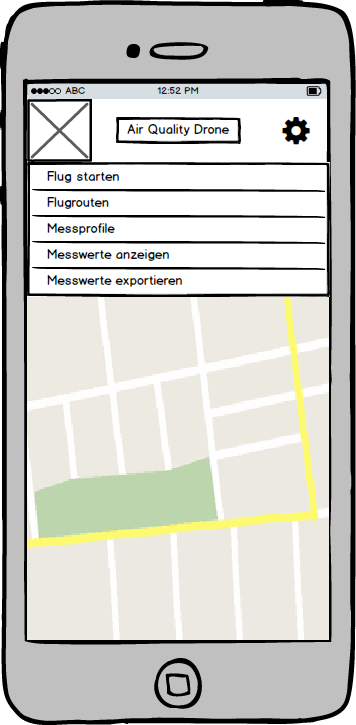
\includegraphics[scale=0.8]{images/Menue}
	\caption{Menü}
\end{figure}
\newpage

\begin{figure}
	\centering
	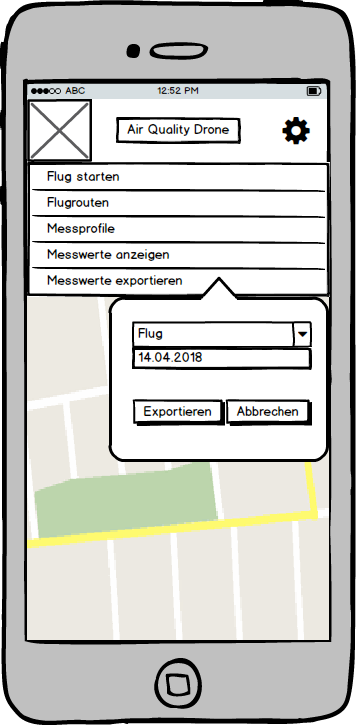
\includegraphics[scale=0.8]{images/MenuePopUp}
	\caption{Menü Pop-Up}
\end{figure}
\newpage

\begin{figure}
	\centering
	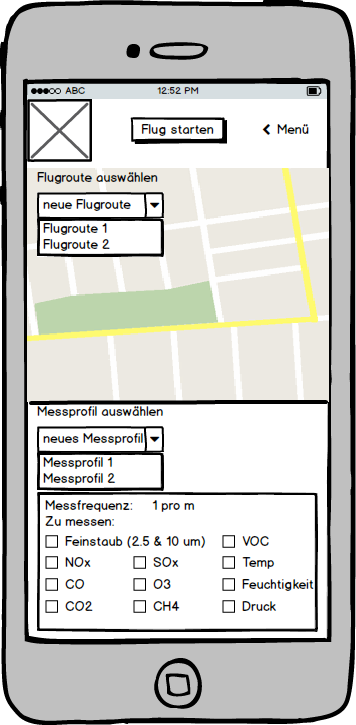
\includegraphics[scale=0.8]{images/FlugStarten}
	\caption{Flug starten}
\end{figure}
\newpage

\begin{figure}
	\centering
	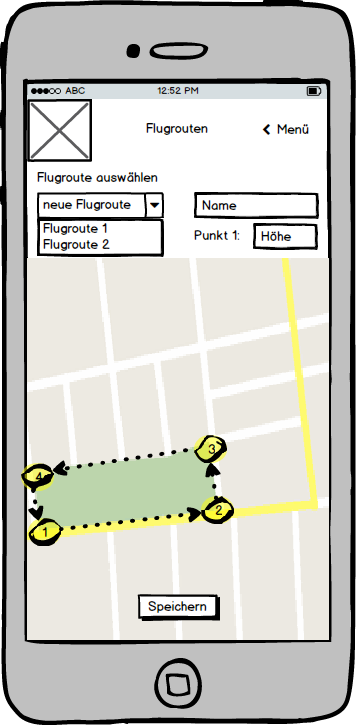
\includegraphics[scale=0.8]{images/Flugrouten}
	\caption{Flugrouten}
\end{figure}
\newpage

\begin{figure}
	\centering
	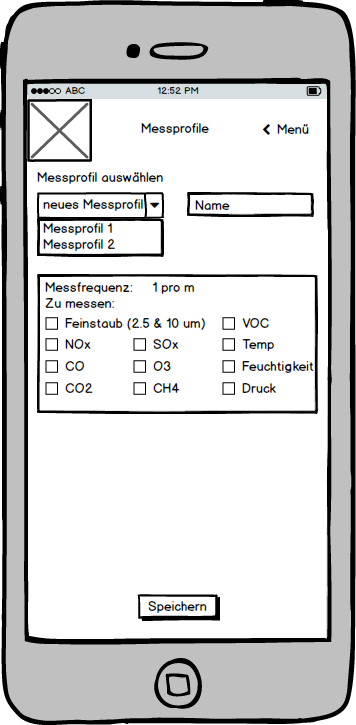
\includegraphics[scale=0.8]{images/Messprofile}
	\caption{Messprofile}
\end{figure}
\newpage

\begin{figure}
	\centering
	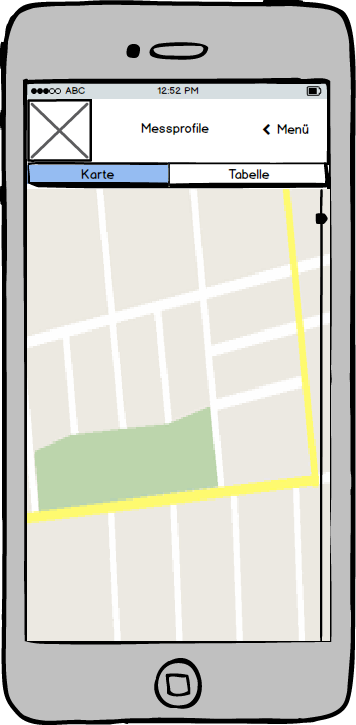
\includegraphics[scale=0.8]{images/MesswerteAnzeigenKarte}
	\caption{Messwerte anzeigen (Karte)}
\end{figure}
\newpage

\begin{figure}
	\centering
	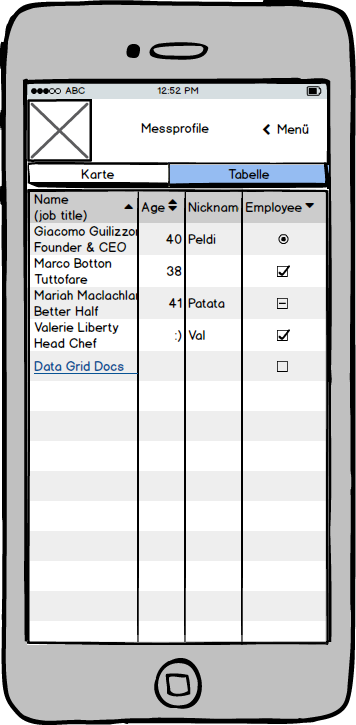
\includegraphics[scale=0.8]{images/MesswerteAnzeigenTabelle}
	\caption{Messwerte anzeigen (Tabelle)}
\end{figure}
\newpage
	
	% Entwicklungsumgebung
	%!TEX root = ../dokumentation.tex



\chapter{Entwicklungsumgebung}\label{cha:Entwicklungsumgebung}

\begin{itemize}
	\item Die App wird mit der Entwicklungsumgebung XCode entwickelt werden.
	\item Die Drohnenaspekte werden mit der Entwicklungsumgebung DJI Mobile SDK
	\item Die Anbindung der Sensoren erfolgt mithilfe des Bosch XDKs und der zugehörigen Entwicklungsumgebung
			
\end{itemize} 
		
	% Abschlussbewertung
	%!TEX root = ../dokumentation.tex



\chapter{Abschlussbewertung}\label{cha:Abschlussbewertung}

	
	
	% Glossar
	\printglossaries %[style=altlist,title=\langglossar]
	
	% sonstiger Anhang
	\clearpage
	\appendix
	% !TeX root = ../dokumentation.tex

\addchap{\langanhang}

{\Large
\begin{enumerate}[label=\Alph*.]
	\item Anforderungsanalyse
	\item Komplettes Schaltungs-Layout
\end{enumerate}
}
\pagebreak

\section*{Anforderungsanalyse}\label{sec:Anforderungsanalyse}

\includepdf[pages=1-34, width=1\textwidth]{Anhang/Anforderungsanalyse.pdf}
\pagebreak
\section*{Komplettes Schaltungs-Layout}\label{sec:Schaltungs-Layout_komplett}
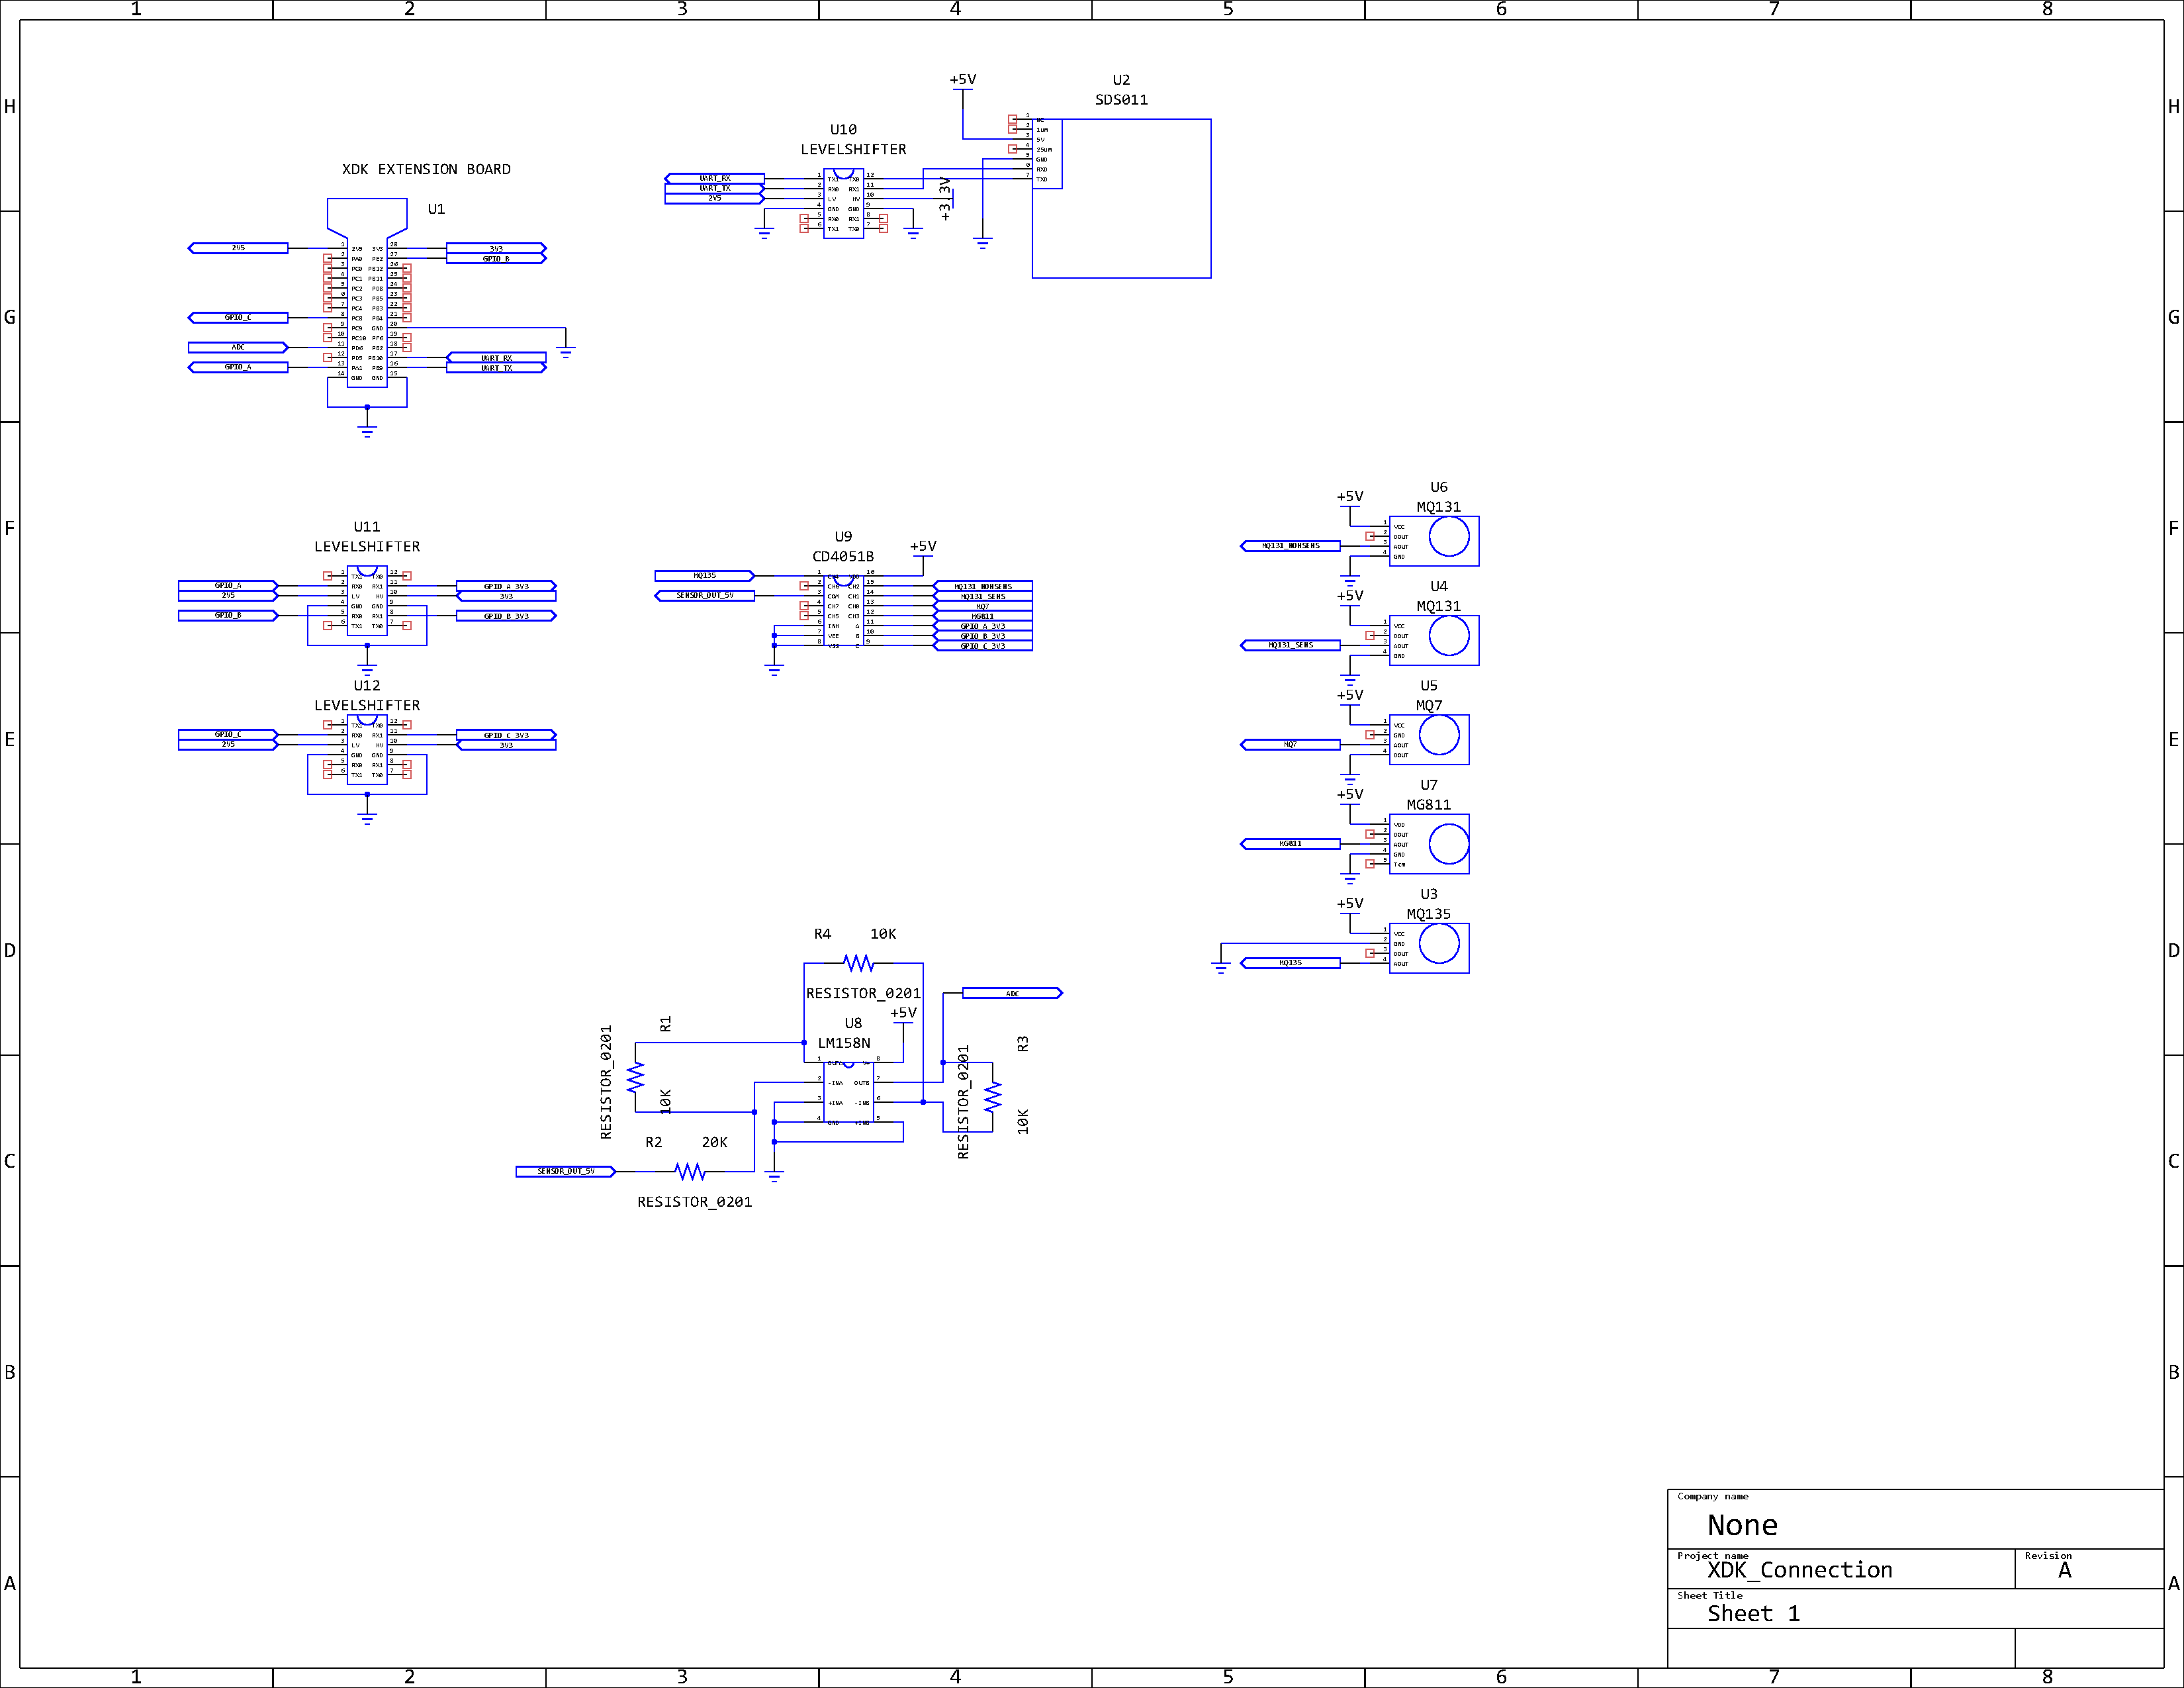
\includepdf[width=\textwidth]{Anhang/XDK_Connection_Schematic.pdf}
\pagebreak


	
\end{document}
